% 動作見本。データはすべて合成。数値は data/sim/mc_summary.csv（Rscript sim/mc_check.R の出力）から写した。
\documentclass[a4paper,10pt]{ltjsarticle}
% 共通プリアンブル。<project>/paper/main.tex から % 共通プリアンブル。<project>/paper/main.tex から % 共通プリアンブル。<project>/paper/main.tex から \input{../../common/lab_preamble}
% 箱は決まったものだけ使う（AGENTS.md §3）。増やすときは AGENTS.md の一覧も直す。
\usepackage{amsmath,amssymb,booktabs,tabularx,longtable,enumitem,xurl,graphicx}
\usepackage[margin=25mm]{geometry}
\usepackage{xcolor}
\usepackage[most]{tcolorbox}
\usepackage{tikz,pgfplots}
\pgfplotsset{compat=1.18}
\usetikzlibrary{arrows.meta,decorations.pathreplacing,positioning,calc}
\usepackage[backend=biber,style=authoryear,natbib=true,maxcitenames=2,doi=true,url=true]{biblatex}
\usepackage[hidelinks]{hyperref}

\definecolor{labBlue}{HTML}{1F5FA8}
\definecolor{labGreen}{HTML}{2E7D4F}
\definecolor{labPurple}{HTML}{6A4C9C}
\definecolor{labOrange}{HTML}{C8641E}
\definecolor{labRed}{HTML}{B03A3A}
\definecolor{labGray}{HTML}{5A6270}

\tcbset{labbase/.style={breakable,enhanced,boxrule=0.6pt,arc=2pt,left=6pt,right=6pt,top=4pt,bottom=4pt,
  fonttitle=\bfseries\small,before skip=8pt,after skip=8pt}}

% 読むための箱
\newtcolorbox{chaptermap}{labbase,colback=labBlue!4,colframe=labBlue,title={この文書の地図}}
\newtcolorbox{keypoint}{labbase,colback=labBlue!4,colframe=labBlue,title={要点}}
\newtcolorbox{term}[1]{labbase,colback=labGray!5,colframe=labGray,title={用語：#1}}
\newtcolorbox{pitfall}{labbase,colback=labRed!4,colframe=labRed,title={落とし穴}}
\newtcolorbox{debate}{labbase,colback=labGray!5,colframe=labGray,title={論争・別の説明}}

% 研究の箱
% 研究仮説：\begin{hypothesis}{H1 短い名前}
\newtcolorbox{hypothesis}[1]{labbase,colback=labGreen!5,colframe=labGreen,title={仮説：#1}}
% 識別戦略：\begin{design}{H1 差の差}
\newtcolorbox{design}[1]{labbase,colback=labBlue!4,colframe=labBlue,title={識別戦略：#1}}
% 推定結果：\begin{result}{H1 の検証（2026-11、確証）}
\newtcolorbox{result}[1]{labbase,colback=labPurple!4,colframe=labPurple,title={結果：#1}}
% 意思決定：続ける／やめる／変える
\newtcolorbox{decision}{labbase,colback=labOrange!6,colframe=labOrange,title={判断（Go/No-Go）}}

% 箱は決まったものだけ使う（AGENTS.md §3）。増やすときは AGENTS.md の一覧も直す。
\usepackage{amsmath,amssymb,booktabs,tabularx,longtable,enumitem,xurl,graphicx}
\usepackage[margin=25mm]{geometry}
\usepackage{xcolor}
\usepackage[most]{tcolorbox}
\usepackage{tikz,pgfplots}
\pgfplotsset{compat=1.18}
\usetikzlibrary{arrows.meta,decorations.pathreplacing,positioning,calc}
\usepackage[backend=biber,style=authoryear,natbib=true,maxcitenames=2,doi=true,url=true]{biblatex}
\usepackage[hidelinks]{hyperref}

\definecolor{labBlue}{HTML}{1F5FA8}
\definecolor{labGreen}{HTML}{2E7D4F}
\definecolor{labPurple}{HTML}{6A4C9C}
\definecolor{labOrange}{HTML}{C8641E}
\definecolor{labRed}{HTML}{B03A3A}
\definecolor{labGray}{HTML}{5A6270}

\tcbset{labbase/.style={breakable,enhanced,boxrule=0.6pt,arc=2pt,left=6pt,right=6pt,top=4pt,bottom=4pt,
  fonttitle=\bfseries\small,before skip=8pt,after skip=8pt}}

% 読むための箱
\newtcolorbox{chaptermap}{labbase,colback=labBlue!4,colframe=labBlue,title={この文書の地図}}
\newtcolorbox{keypoint}{labbase,colback=labBlue!4,colframe=labBlue,title={要点}}
\newtcolorbox{term}[1]{labbase,colback=labGray!5,colframe=labGray,title={用語：#1}}
\newtcolorbox{pitfall}{labbase,colback=labRed!4,colframe=labRed,title={落とし穴}}
\newtcolorbox{debate}{labbase,colback=labGray!5,colframe=labGray,title={論争・別の説明}}

% 研究の箱
% 研究仮説：\begin{hypothesis}{H1 短い名前}
\newtcolorbox{hypothesis}[1]{labbase,colback=labGreen!5,colframe=labGreen,title={仮説：#1}}
% 識別戦略：\begin{design}{H1 差の差}
\newtcolorbox{design}[1]{labbase,colback=labBlue!4,colframe=labBlue,title={識別戦略：#1}}
% 推定結果：\begin{result}{H1 の検証（2026-11、確証）}
\newtcolorbox{result}[1]{labbase,colback=labPurple!4,colframe=labPurple,title={結果：#1}}
% 意思決定：続ける／やめる／変える
\newtcolorbox{decision}{labbase,colback=labOrange!6,colframe=labOrange,title={判断（Go/No-Go）}}

% 箱は決まったものだけ使う（AGENTS.md §3）。増やすときは AGENTS.md の一覧も直す。
\usepackage{amsmath,amssymb,booktabs,tabularx,longtable,enumitem,xurl,graphicx}
\usepackage[margin=25mm]{geometry}
\usepackage{xcolor}
\usepackage[most]{tcolorbox}
\usepackage{tikz,pgfplots}
\pgfplotsset{compat=1.18}
\usetikzlibrary{arrows.meta,decorations.pathreplacing,positioning,calc}
\usepackage[backend=biber,style=authoryear,natbib=true,maxcitenames=2,doi=true,url=true]{biblatex}
\usepackage[hidelinks]{hyperref}

\definecolor{labBlue}{HTML}{1F5FA8}
\definecolor{labGreen}{HTML}{2E7D4F}
\definecolor{labPurple}{HTML}{6A4C9C}
\definecolor{labOrange}{HTML}{C8641E}
\definecolor{labRed}{HTML}{B03A3A}
\definecolor{labGray}{HTML}{5A6270}

\tcbset{labbase/.style={breakable,enhanced,boxrule=0.6pt,arc=2pt,left=6pt,right=6pt,top=4pt,bottom=4pt,
  fonttitle=\bfseries\small,before skip=8pt,after skip=8pt}}

% 読むための箱
\newtcolorbox{chaptermap}{labbase,colback=labBlue!4,colframe=labBlue,title={この文書の地図}}
\newtcolorbox{keypoint}{labbase,colback=labBlue!4,colframe=labBlue,title={要点}}
\newtcolorbox{term}[1]{labbase,colback=labGray!5,colframe=labGray,title={用語：#1}}
\newtcolorbox{pitfall}{labbase,colback=labRed!4,colframe=labRed,title={落とし穴}}
\newtcolorbox{debate}{labbase,colback=labGray!5,colframe=labGray,title={論争・別の説明}}

% 研究の箱
% 研究仮説：\begin{hypothesis}{H1 短い名前}
\newtcolorbox{hypothesis}[1]{labbase,colback=labGreen!5,colframe=labGreen,title={仮説：#1}}
% 識別戦略：\begin{design}{H1 差の差}
\newtcolorbox{design}[1]{labbase,colback=labBlue!4,colframe=labBlue,title={識別戦略：#1}}
% 推定結果：\begin{result}{H1 の検証（2026-11、確証）}
\newtcolorbox{result}[1]{labbase,colback=labPurple!4,colframe=labPurple,title={結果：#1}}
% 意思決定：続ける／やめる／変える
\newtcolorbox{decision}{labbase,colback=labOrange!6,colframe=labOrange,title={判断（Go/No-Go）}}

\addbibresource{../common/refs.bib}

\title{動作見本：系列相関のあるパネルで、単純な差の差は偽陽性率を保つが、効果0.3は検出できない}
\author{AI ネイティブ経済学ラボ（見本）}
\date{2026年11月14日（最終更新）}

\begin{document}
\maketitle

\begin{abstract}
これはラボの仕組みを見せるための見本であり、データはすべて合成である。
200単位×10期の合成パネルで、差の差の手続きを2通り点検した。
真の効果が0のときの棄却率は、単位ごとの前後差で6.2\%、観測を独立とみなす OLS で6.4\%だった（各500回）。
「独立とみなす OLS は偽陽性が増える」という事前の予想（H2）は、この設定では外れた。
効果0.3での検出力は66.8\%で、80\%に届かなかった。
\end{abstract}

\begin{chaptermap}
\textbf{3行でいうと}
\begin{enumerate}[leftmargin=*]
  \item 背景：分析コードを実データに当てる前に、答えの分かっている合成データで手続きを確かめる（段階6）。
  \item 仮説：H1 偽陽性率は保たれる、H2 独立とみなすと偽陽性が増える、H3 効果0.3を検出できる。
  \item 現状：H1 支持、H2 棄却、H3 棄却。未ロック。結果はすべて合成データの区分である。
\end{enumerate}
\end{chaptermap}

%======================================================================
\section{背景と問い}\label{sec:demo-bg}
差の差では、同じ単位を何期も観測する。誤差が時間を通じて相関していると、観測を独立とみなした標準誤差は信用できない場合がある。
どの程度ずれるかは、設定（期の数、処置の時点、相関の強さ）に依存する。
だから、自分のデータと同じ構造の合成データで確かめる。

\begin{term}{偽陽性率と検出力}
偽陽性率は、真の効果が0なのに「効果あり」と判定する割合である。5\%水準の検定なら5\%が目標になる。
検出力は、真の効果があるときに「効果あり」と判定できる割合である。80\%を目安にすることが多い。
\end{term}

%======================================================================
\section{先行研究}\label{sec:demo-prior}
見本なので、文献調査はしていない。実プロジェクトでは、ここに転換点の論文5〜10本の表を置く。
関連する方法論の文献として、事前に決めることの利点と限界\parencite{olken2015}、
検定を通過した後の推定の歪み\parencite{roth2022}、仕様を網羅して示す方法\parencite{simonsohn2020}、
有意な結果への偏りの実態\parencite{brodeur2020}がある。

%======================================================================
\section{研究仮説}\label{sec:demo-hyp}

\begin{hypothesis}{H1 単位ごとの前後差は偽陽性率を保つ}
\textbf{仮説}：真の効果が0のとき、5\%水準の検定が棄却する割合は3〜7\%に収まる。\\
\textbf{成功基準}：棄却率が0.03以上0.07以下（500回での標準誤差は約0.01）。\\
\textbf{棄却条件}：棄却率が0.03未満または0.07超。\\
\textbf{状態}：支持（2026-11-14）。ただし基準は結果を見た後に書いた。
\end{hypothesis}

\begin{hypothesis}{H2 独立とみなす OLS は偽陽性が増える}
\textbf{仮説}：真の効果が0のとき、棄却率は7\%を超える。\\
\textbf{根拠}：系列相関があると標準誤差が小さくなりすぎる、という筆者の事前の予想。\\
\textbf{成功基準}：棄却率が0.07超。\quad\textbf{棄却条件}：棄却率が0.07以下。\\
\textbf{状態}：棄却（2026-11-14）。この仮説だけが、結果を見る前に立てたものである。
\end{hypothesis}

\begin{hypothesis}{H3 効果0.3を検出力80\%で検出できる}
\textbf{仮説}：真の効果0.3での棄却率は80\%以上になる。\\
\textbf{成功基準}：棄却率が0.80以上。\quad\textbf{棄却条件}：棄却率が0.80未満。\\
\textbf{状態}：棄却（2026-11-14）。基準は結果を見た後に書いた。
\end{hypothesis}

%======================================================================
\section{データ}\label{sec:demo-data}
合成パネルを \texttt{sim/mc\_check.R} で生成する。単位は200、期は10、第6期から処置、処置群は半数である。
結果変数は式\ref{eq:demo-dgp}で作る。乱数の種は20261114である。
\begin{equation}
  y_{it} = \alpha_i + 0.05\,t + \tau D_{it} + \varepsilon_{it}, \qquad
  \varepsilon_{it} = 0.6\,\varepsilon_{i,t-1} + u_{it}
  \label{eq:demo-dgp}
\end{equation}
$\alpha_i$ は標準偏差1の単位固定効果、$\varepsilon_{it}$ は標準偏差1の誤差、$D_{it}$ は処置群の処置後で1をとる。
真の効果 $\tau$ は0、0.1、0.2、0.3、0.5の5通りを試す。

%======================================================================
\section{識別戦略と推定}\label{sec:demo-design}

\begin{design}{2つの手続き}
\textbf{単位ごとの前後差（did\_unit）}：単位ごとに「処置後の平均−処置前の平均」を取り、処置群と対照群の平均の差を推定値とする。標準誤差は単位を独立とみなして計算する。\\
\textbf{独立とみなす OLS（naive\_ols）}：単位×期の2000観測に、処置群・処置後・交差項を入れた OLS を当て、通常の標準誤差を使う。\\
\textbf{評価}：各設定で500回くり返し、偏り・95\%信頼区間の被覆率・棄却率を測る。\\
\textbf{推論}：棄却率0.05のモンテカルロ標準誤差は $\sqrt{0.05\times0.95/500}\approx0.01$ である。
\end{design}

%======================================================================
\section{予想される結果}\label{sec:demo-expected}
シミュレーションの前に筆者が予想していたのは、H2（独立とみなす OLS の棄却率が7\%を超える）だけである。
H1 と H3 の数値基準は、結果を見た後に書いた。したがって、確証と呼べるのは H2 の判定だけである。

%======================================================================
\section{結果}\label{sec:demo-result}

\begin{result}{H1・H2 の点検（2026-11-14、合成データ）}
\textbf{何をした}：真の効果0で500回。\\
\textbf{何が分かった}：棄却率は did\_unit で0.062、naive\_ols で0.064。被覆率は0.938と0.936（表\ref{tab:demo-mc}）。\\
\textbf{判定}：H1 は支持（0.03〜0.07の範囲内）。H2 は棄却（0.07を超えなかった）。
\end{result}

\begin{result}{H3 の点検（2026-11-14、合成データ）}
\textbf{何をした}：真の効果0.3で500回。\\
\textbf{何が分かった}：did\_unit の棄却率は0.668。効果0.5では0.974（図\ref{fig:demo-power}）。\\
\textbf{判定}：H3 は棄却。検出力80\%に届く効果は0.3と0.5の間にある。
\end{result}

\begin{table}[htbp]
\centering\small
\begin{tabular}{llrrrr}
\toprule
真の効果 & 手続き & 偏り & 標準誤差の平均 & 被覆率 & 棄却率 \\
\midrule
0 & did\_unit & 0.0005 & 0.1255 & 0.938 & 0.062 \\
0 & naive\_ols & 0.0005 & 0.1260 & 0.936 & 0.064 \\
\midrule
0.1 & did\_unit & 0.0045 & 0.1259 & 0.938 & 0.134 \\
0.2 & did\_unit & $-0.0032$ & 0.1254 & 0.958 & 0.332 \\
0.3 & did\_unit & $-0.0046$ & 0.1256 & 0.948 & 0.668 \\
0.5 & did\_unit & $-0.0045$ & 0.1257 & 0.952 & 0.974 \\
\bottomrule
\end{tabular}
\caption{シミュレーションの結果（各500回、合成データ）。全行は \texttt{data/sim/mc\_summary.csv}。}
\label{tab:demo-mc}
\end{table}

\begin{figure}[htbp]
\centering
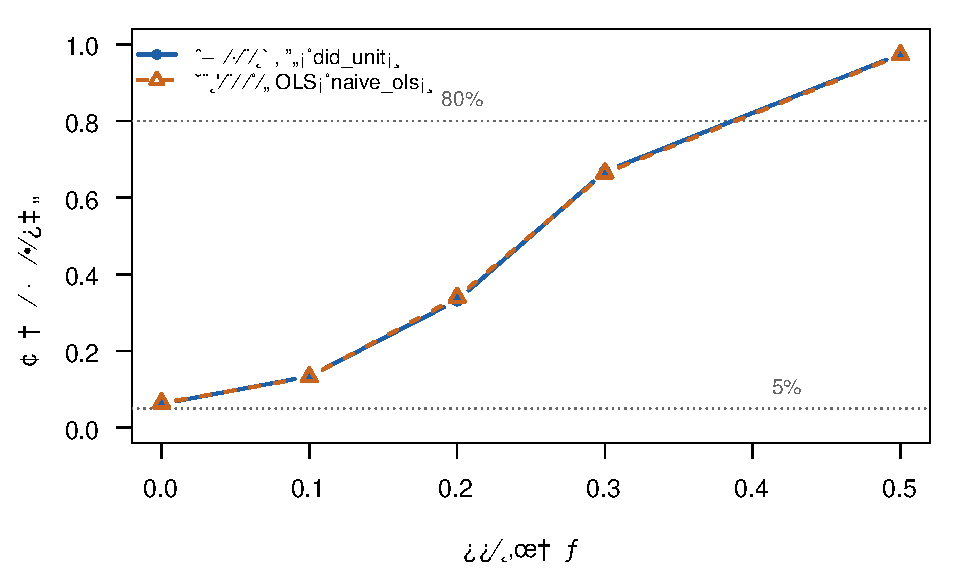
\includegraphics[width=0.8\linewidth]{figs/demo_power.pdf}
\caption{真の効果ごとの棄却率（各500回、合成データ）。効果0での値が偽陽性率、それ以外が検出力である。2つの手続きはほぼ重なる。データは \texttt{data/sim/mc\_summary.csv}、作図は \texttt{code/02\_figs.R}。}
\label{fig:demo-power}
\end{figure}

%======================================================================
\section{考察}\label{sec:demo-discussion}
H2 が外れた理由は、設定にあると考えられる（筆者の見解、未検証）。
この設定では、処置前と処置後が5期ずつで、処置群と対照群が同数である。
単位固定効果は前後差で消え、系列相関は前後の平均の差のばらつきを小さくする方向に働く。
2つの効果が打ち消し合い、独立とみなした標準誤差がたまたま合った可能性がある。
期の数や相関の強さを変えれば、結論は変わりうる。

\begin{pitfall}
「この設定で問題が出なかった」は、「この手続きは安全だ」を意味しない。
確かめたのは1つの設定だけである。自分のデータの構造に合わせて \texttt{PARAMS} を書き換え、もう一度測る必要がある。
\end{pitfall}

%======================================================================
\section{判断と次の一手}\label{sec:demo-decision}
\begin{decision}
\textbf{結論}：見本として完了。研究としては進めない。\\
\textbf{理由}：仕組み（仮説の箱、結果の箱、仕様の記録、R と Python の照合）が端から端まで動くことを確かめるのが目的だった。\\
\textbf{次の一手}：実プロジェクトでは \texttt{\_template} をコピーし、段階4の終わりに人が承認してロックする。
\end{decision}

\section*{更新履歴}
\begin{itemize}
  \item 2026-11-14：作成。H2 は事前の予想、H1 と H3 の基準は結果を見た後に追加。
\end{itemize}

\printbibliography[title={参考文献}]
\end{document}
